% ------------------------------------------------------------------------------
% TYPO3 CMS 8.1 - What's New - Chapter "Introduction" (German Version)
%
% @author	Michael Schams <schams.net>
% @license	Creative Commons BY-NC-SA 3.0
% @link		http://typo3.org/download/release-notes/whats-new/
% @language	German
% ------------------------------------------------------------------------------
% LTXE-CHAPTER-UID:		67d83fb2-68e46798-3e745e9b-074bce01
% LTXE-CHAPTER-NAME:	Introduction
% ------------------------------------------------------------------------------

\section{Introduction}
\begin{frame}[fragile]
	\frametitle{Introduction}

	\begin{center}\huge{Einführung}\end{center}
	\begin{center}\huge{\color{typo3darkgrey}\textbf{Die Fakten}}\end{center}

\end{frame}

% ------------------------------------------------------------------------------
% LTXE-SLIDE-START
% LTXE-SLIDE-UID:		4aae926b-8f438557-93006bce-fbde33df
% LTXE-SLIDE-ORIGIN:	de1d09f3-1b80b171-45e65f78-cbf750bc English
% LTXE-SLIDE-TITLE:		TYPO3 CMS 8.1 - The Facts
% ------------------------------------------------------------------------------
\begin{frame}[fragile]
	\frametitle{Einführung}
	\framesubtitle{TYPO3 CMS 8.1 - Die Fakten}

	\begin{itemize}
		\item Veröffentlichungsdatum: 3 Mai 2016
		\item Releasetyp: Sprint Release
		\item Vision: Tightening the screws
	\end{itemize}

	\begin{figure}
		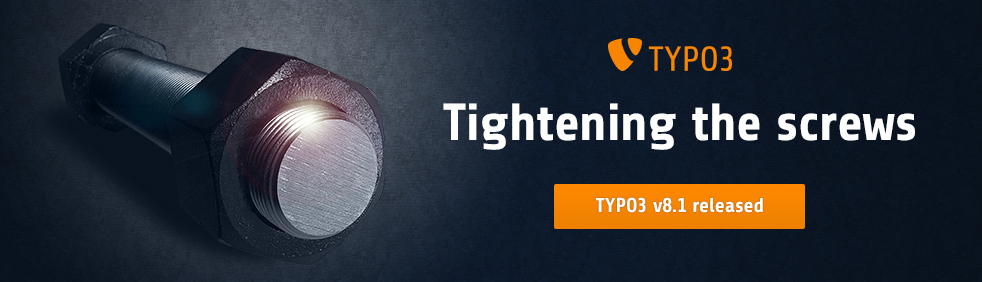
\includegraphics[width=0.95\linewidth]{Introduction/typo3cms81-banner.png}
	\end{figure}

\end{frame}

% ------------------------------------------------------------------------------
% LTXE-SLIDE-START
% LTXE-SLIDE-UID:		409070dd-30efb126-c7f51ea7-bbb33fd5
% LTXE-SLIDE-ORIGIN:	29730fa0-cfb7b672-9541b86e-5d979dcc English
% LTXE-SLIDE-TITLE:		System Requirements
% ------------------------------------------------------------------------------
\begin{frame}[fragile]
	\frametitle{Einführung}
	\framesubtitle{Systemvoraussetzungen}

	\begin{itemize}
		\item PHP:\tabto{3cm}Version 7
		\item MySQL:\tabto{3cm}Version 5.5 - 5.7
		\item Festplattenplatz:\tabto{3cm}mindestens 200 MB
		\item PHP Einstellungen:

			\begin{itemize}
				\item \texttt{memory\_limit} >= 128M
				\item \texttt{max\_execution\_time} >= 240s
				\item \texttt{max\_input\_vars} >= 1500
				\item PHP Kompilierungsoption \texttt{--disable-ipv6} darf \underline{nicht} aktiviert sein
			\end{itemize}

		\item Das Backend benötigt einen Microsoft Internet Explorer 11 oder später,
			Microsoft Edge, Google Chrome, Firefox, Safari oder jeden anderen modernen Browser

	\end{itemize}

\end{frame}

% ------------------------------------------------------------------------------
% LTXE-SLIDE-START
% LTXE-SLIDE-UID:		c941167f-36d1b696-9de0471c-3f59706a
% LTXE-SLIDE-ORIGIN:	c5361815-a40c49e2-c6fe93fe-0e0b9466 English
% LTXE-SLIDE-TITLE:		Development And Release Timeline
% ------------------------------------------------------------------------------
\begin{frame}[fragile]
	\frametitle{Einführung}
	\framesubtitle{Release Zyklus}

	\begin{figure}
		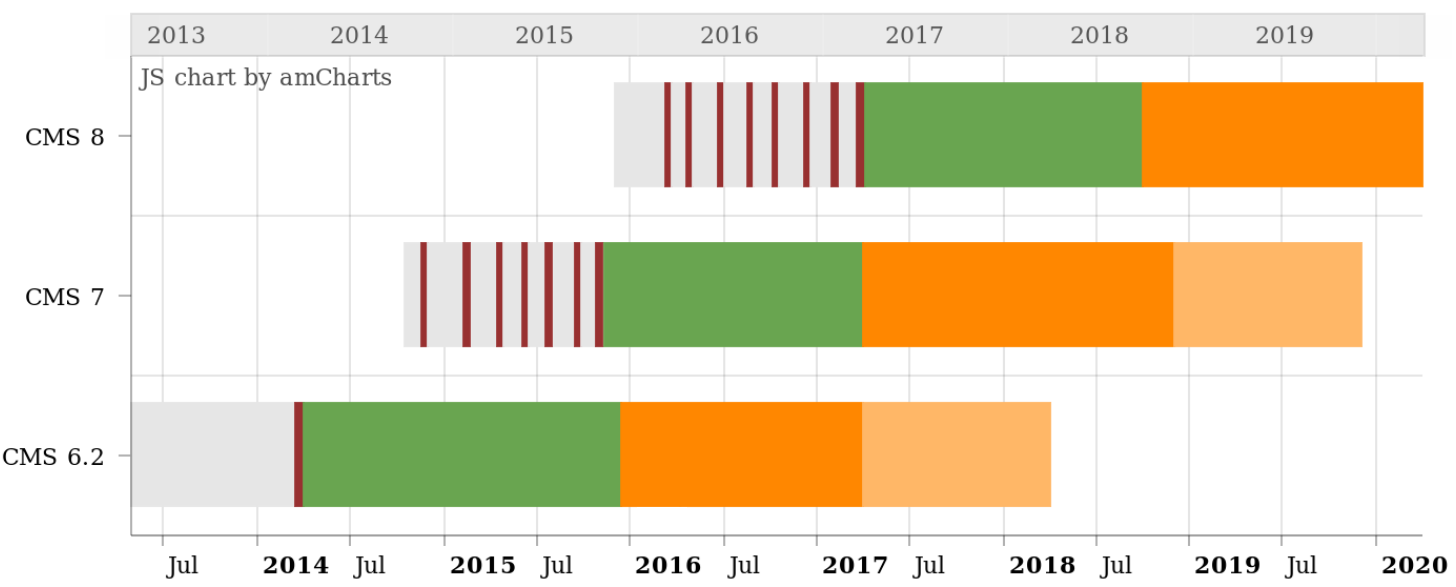
\includegraphics[width=1\linewidth]{Introduction/ReleaseAgenda.png}
	\end{figure}

\end{frame}

% ------------------------------------------------------------------------------
% LTXE-SLIDE-START
% LTXE-SLIDE-UID:		88aa00e2-8f024769-e2eec887-7fa9aaea
% LTXE-SLIDE-ORIGIN:	99e5aeb9-52a34013-e7784c4c-9ff8f701 English
% LTXE-SLIDE-TITLE:		TYPO3 CMS Roadmap
% ------------------------------------------------------------------------------
\begin{frame}[fragile]
	\frametitle{Einführung}
	\framesubtitle{TYPO3 CMS Roadmap}

	Voraussichtliche Veröffentlichungen und deren Hauptfokus:

	\begin{itemize}

		\item v8.0 \tabto{1.1cm}22/Mär/2016\tabto{3.4cm}Adding last minute things
		\item
			\begingroup
				\color{typo3orange}
					v8.1 \tabto{1.1cm}03/Mai/2016\tabto{3.4cm}Cloud Integration
			\endgroup
		\item v8.2 \tabto{1.1cm}05/Jul/2016\tabto{3.4cm}Rich Text Editor
		\item v8.3 \tabto{1.1cm}30/Aug/2016\tabto{3.4cm}Frontend Editing on Steroids
		\item v8.4 \tabto{1.1cm}18/Okt/2016\tabto{3.4cm}\textit{to be determined}
		\item v8.5 \tabto{1.1cm}20/Dez/2016\tabto{3.4cm}Integrator Support
		\item v8.6 \tabto{1.1cm}14/Feb/2017\tabto{3.4cm}\textit{to be determined}
		\item v8.7 \tabto{1.1cm}04/Apr/2017\tabto{3.4cm}LTS Preparation

	\end{itemize}

	\smaller
		\url{https://typo3.org/typo3-cms/roadmap/}\newline
		\url{https://typo3.org/news/article/kicking-off-typo3-v8-development/}
	\normalsize

\end{frame}

% ------------------------------------------------------------------------------
% LTXE-SLIDE-START
% LTXE-SLIDE-UID:		9d52a518-7ba22c0e-5dde2ad3-82a6407e
% LTXE-SLIDE-ORIGIN:	3159ba35-9542333b-a0495cfc-af0010a5 English
% LTXE-SLIDE-TITLE:		Installation
% ------------------------------------------------------------------------------
\begin{frame}[fragile]
	\frametitle{Einführung}
	\framesubtitle{Installation}

	\begin{itemize}
		\item Empfohlene Installationsschritte unter Linux/Mac OS X\newline
			(DocumentRoot ist beispielsweise \texttt{/var/www/site/htdocs}):
		\begin{lstlisting}
			$ cd /var/www/site
			$ wget --content-disposition get.typo3.org/8.1
			$ tar xzf typo3_src-8.1.0.tar.gz
			$ cd htdocs
			$ ln -s ../typo3_src-8.1.0 typo3_src
			$ ln -s typo3_src/index.php
			$ ln -s typo3_src/typo3
			$ touch FIRST_INSTALL
		\end{lstlisting}

		\item Symbolische Links unter Microsoft Windows:

			\begin{itemize}
				\item unter Windows XP/2000 kann \texttt{junction} benutzt werden
				\item unter Windows Vista und Windows 7 kann \texttt{mklink} benutzt werden
			\end{itemize}

	\end{itemize}
\end{frame}

% ------------------------------------------------------------------------------
% LTXE-SLIDE-START
% LTXE-SLIDE-UID:		1328c049-6f26e75a-adfae447-e9191d4e
% LTXE-SLIDE-ORIGIN:	d3497bd8-61e5242f-0009b322-3a285ed7 English
% LTXE-SLIDE-TITLE:		Upgrade to TYPO3 CMS 7
% ------------------------------------------------------------------------------
\begin{frame}[fragile]
	\frametitle{Einführung}
	\framesubtitle{Upgrade zu TYPO3 CMS 8.x}

	\begin{itemize}
		\item Upgrade ist nur möglich von TYPO3 CMS 7.6 LTS
		\item TYPO3 CMS < 7.6 LTS sollte zuerst auf TYPO3 CMS 7.6 LTS aktualisiert werden
	\end{itemize}

	\begin{itemize}

		\item Upgrade-Anleitung:\newline
			\smaller\url{http://wiki.typo3.org/Upgrade#Upgrading_to_8.1}\normalsize
		\item Official TYPO3 guide "TYPO3 Installation and Upgrading":
			\smaller\url{http://docs.typo3.org/typo3cms/InstallationGuide}\normalsize
		\item Generelles Vorgehen:
			\begin{itemize}
				\item Prüfen, ob Mindestvoraussetzungen erfüllt sind \small(PHP, MySQL, etc.)
				\item Das \textbf{deprecation\_*.log} der TYPO3 Instanz durchsehen
				\item Sämtliche Extensions auf den aktuellsten Stand bringen
				\item Neuen TYPO3 Quellcode entpacken und im Install Tool den Upgrade Wizard ausführen
				\item Startup Modul von Backend Benutzern überprüfen (optional)
			\end{itemize}
	\end{itemize}

\end{frame}

% ------------------------------------------------------------------------------
